% Biên dịch bằng XeLaTeX. Nội dung được tách theo phần để dễ sửa.
\documentclass[12pt,a4paper]{extarticle}
% extarticle không có tùy chọn 13pt; đặt thực sự 13pt để tránh bị bỏ qua.
\makeatletter
\renewcommand\normalsize{\@setfontsize\normalsize{13pt}{15.6pt}}
\makeatother
\normalsize
\usepackage{fontspec}
\IfFontExistsTF{Times New Roman}{\setmainfont{Times New Roman}}{\setmainfont{Liberation Serif}}
\setsansfont{Liberation Sans}
\setmonofont[Scale=0.78]{Liberation Mono}
\usepackage[top=2cm,bottom=2cm,left=2.5cm,right=2cm]{geometry}
\usepackage{setspace}
\setstretch{1.4}
\usepackage{amsmath,amssymb,graphicx,booktabs,tabularx,array,float}
\usepackage{unicode-math}
\setmathfont{latinmodern-math.otf}
\usepackage{etoolbox}
\AtBeginEnvironment{table}{\setstretch{1.1}}
\usepackage{tikz}
\usetikzlibrary{arrows.meta,positioning,calc}
\usepackage{enumitem,caption,fancyhdr,titlesec,microtype}
\usepackage[hidelinks,unicode,hypertexnames=false]{hyperref}
\hypersetup{pdftitle={So sánh RAG truyền thống và GraphRAG trong hỏi đáp có dẫn nguồn về quy chế đào tạo của HaUI},pdfauthor={Trần Trung Hiếu},pdfsubject={Nghiên cứu thực nghiệm thăm dò RAG và GraphRAG}}
\renewcommand{\contentsname}{MỤC LỤC}
\renewcommand{\refname}{TÀI LIỆU THAM KHẢO}
\renewcommand{\figurename}{Hình}
\renewcommand{\tablename}{Bảng}
\captionsetup{font=small,labelfont=bf}
\setlength{\parindent}{1cm}
\setlength{\parskip}{3pt}
\setlength{\emergencystretch}{2em}
\setlist[itemize]{leftmargin=1.4cm,itemsep=2pt,topsep=4pt}
\setlist[enumerate]{leftmargin=1.4cm,itemsep=2pt,topsep=4pt}
\renewcommand{\arraystretch}{1.2}
\titleformat{\section}{\large\bfseries}{\thesection.}{.5em}{}
\titleformat{\subsection}{\normalsize\bfseries}{\thesubsection.}{.5em}{}
\titlespacing*{\section}{0pt}{8pt}{8pt}
\titlespacing*{\subsection}{0pt}{7pt}{4pt}
\pagestyle{fancy}
\fancyhf{}
\fancyhead[L]{\small Nghiên cứu RAG và GraphRAG}
\fancyhead[R]{\small Trần Trung Hiếu}
\fancyfoot[C]{\thepage}
\setlength{\headheight}{16pt}
\newcommand{\code}[1]{{\ttfamily\expandafter\nolinkurl\expandafter{\detokenize{#1}}}}
\newcommand{\sourcefile}[1]{\par\noindent{\footnotesize Nguồn số liệu: \code{#1}.}\par}
\newcommand{\blankfield}{\rule{5.1cm}{0.3pt}}
\begin{document}
\begin{titlepage}
\thispagestyle{empty}
\begin{tikzpicture}[remember picture,overlay]
\draw[blue!55!black,line width=2pt] ($(current page.north west)+(1.5cm,-1.5cm)$) rectangle ($(current page.south east)+(-1.5cm,1.5cm)$);
\draw[blue!55!black,line width=.6pt] ($(current page.north west)+(1.65cm,-1.65cm)$) rectangle ($(current page.south east)+(-1.65cm,1.65cm)$);
\end{tikzpicture}
\centering
\vspace*{.9cm}
{\fontsize{15}{21}\selectfont\bfseries TRƯỜNG ĐẠI HỌC CÔNG NGHIỆP HÀ NỘI\par}
\vspace{.35cm}
{\fontsize{14}{20}\selectfont KHOA: \rule{6cm}{.3pt}\par}
\vspace{2cm}
{\fontsize{19}{27}\selectfont\bfseries BÁO CÁO NGHIÊN CỨU KHOA HỌC\par}
\vspace{.3cm}
{\fontsize{14}{20}\selectfont DỰ ÁN CÁ NHÂN\par}
\vspace{1.1cm}
{\fontsize{18}{26}\selectfont\bfseries SO SÁNH RAG TRUYỀN THỐNG VÀ GRAPHRAG TRONG HỎI ĐÁP CÓ DẪN NGUỒN VỀ QUY CHẾ ĐÀO TẠO CỦA TRƯỜNG ĐẠI HỌC CÔNG NGHIỆP HÀ NỘI\par}
\vspace{1.6cm}
\begin{tabular}{ll}
Sinh viên thực hiện: & \textbf{Trần Trung Hiếu}\\[.35cm]
Mã sinh viên: & \blankfield\\[.35cm]
Lớp: & \blankfield\\[.35cm]
Giảng viên hướng dẫn: & \blankfield\\[.35cm]
Đơn vị/bộ môn: & \blankfield
\end{tabular}
\vfill
{\fontsize{14}{20}\selectfont Hà Nội, tháng \rule{1cm}{.3pt} năm \rule{1.3cm}{.3pt}\par}
\vspace{.7cm}
\end{titlepage}
\pagenumbering{roman}
\setcounter{tocdepth}{1}
\tableofcontents
\clearpage
\section*{TÓM TẮT}
\addcontentsline{toc}{section}{Tóm tắt}
Đề tài so sánh RAG truyền thống dùng truy xuất vector với GraphRAG tùy biến kết hợp ngữ nghĩa, từ vựng và quan hệ văn bản trong hỏi đáp quy chế đào tạo HaUI. Một đối chứng hybrid không đồ thị được bổ sung ở tầng truy xuất. Mục tiêu là tìm đúng chứng cứ, trả lời đúng phạm vi và phân tích lỗi theo loại câu hỏi.

Tập dữ liệu gồm 9 PDF từ các trang chính thức của HaUI, được lập thành 449 đoạn; 313 đoạn lấy từ bản OCR và 136 đoạn lấy từ PDF có lớp chữ. Đồ thị có 480 nút, 1.872 cạnh, trong đó 22 quan hệ pháp lý có câu dẫn được đối chiếu với trang và đoạn chỉ mục. Phép thử ngày 01/10/2026 gồm 174 lượt truy xuất trên ba bộ nội bộ có chồng lấp và 40 yêu cầu Gemini cho 20 cặp câu hỏi. Hai hệ thống sinh sử dụng cùng model \code{gemini-3.5-flash-lite}, prompt, giới hạn chứng cứ và cấu hình đầu ra.

Ở bộ 30 câu ban đầu, Recall@5 của RAG và GraphRAG lần lượt là 0,74 và 0,78; số câu tìm đủ chứng cứ là 17/25 và 16/25. Trên bộ 8 câu quan hệ, Recall@5 tăng từ 0,25 của RAG lên 0,625 của hybrid và 1,00 của GraphRAG. Với 16 câu có đáp án trong bộ sinh, số câu đúng ý chính là 8 và 11; số câu đủ ý là 4 và 8. Cả hai từ chối phù hợp 4 câu ngoài corpus. Điểm nội dung là đánh giá sơ bộ bằng trợ lý AI, chưa được chấm độc lập bởi con người.

Phân tích trường hợp cho thấy GraphRAG hữu ích khi câu hỏi yêu cầu quan hệ sửa đổi, thay thế hoặc xác định phiên bản. Tuy nhiên, hệ thống vẫn chọn sai phạm vi ở một câu về thang điểm; cả hai bỏ lỡ điều kiện ở câu hỏi nhiều điều. Kiểm định cặp thăm dò cho $p=0{,}4531$, chưa cung cấp bằng chứng đủ mạnh về ưu thế chung. Kết quả phục vụ phân tích nguyên nhân và thiết kế đánh giá tiếp theo, không khẳng định hiệu lực hiện hành của toàn bộ corpus hoặc khả năng tổng quát trên dữ liệu độc lập.

\noindent\textbf{Từ khóa:} RAG; GraphRAG; hỏi đáp có dẫn nguồn; quy chế đào tạo; OCR; đánh giá truy xuất.

\noindent\textbf{Thuật ngữ:} corpus là tập chứng cứ; gold là đáp án/ID tham chiếu; chunk là đoạn chỉ mục; trace là dấu vết truy xuất; OCR là nhận dạng chữ từ ảnh; RPM là số yêu cầu API mỗi phút.

\clearpage
\pagenumbering{arabic}
\section{Giới thiệu và mục tiêu nghiên cứu}
\subsection{Bài toán}
Quy định đào tạo phân tán giữa quy chế chung, đánh giá, khóa luận, chuẩn đầu ra và quyết định sửa đổi. Người tra cứu cần đúng nội dung, đối tượng và phiên bản. Tìm một đoạn gần nghĩa có thể bỏ qua điều kiện ở khoản khác hoặc nhầm cách quy đổi điểm với khoảng điểm.

Citation giúp mở lại trang gốc, nhưng ID có thật chưa bảo đảm phát biểu được hỗ trợ. Bài toán gồm truy xuất, sinh nội dung và từ chối khi corpus thiếu thông tin. Đối tượng nghiên cứu là nguyên mẫu trên tài liệu HaUI đã thu thập, ở quy mô dự án cá nhân cấp trường.

\subsection{Câu hỏi nghiên cứu}
\begin{enumerate}
\item Khi giữ chung corpus và số đoạn đầu ra, GraphRAG thay đổi khả năng tìm chứng cứ như thế nào so với RAG vector và hybrid không đồ thị?
\item Lợi ích quan sát được tập trung ở câu hỏi một điều, nhiều điều, phiên bản hay quan hệ văn bản?
\item Chất lượng đáp án có đi cùng Recall@5 hay còn bị chi phối bởi phạm vi, điều kiện và cách mô hình sinh sử dụng chứng cứ?
\item Độ trễ và lượng token thay đổi ra sao trong phép thử nhỏ, và dữ liệu hiện có cho phép kết luận đến đâu?
\end{enumerate}

\subsection{Phạm vi và đóng góp}
Phạm vi gồm 9 PDF chính thức của HaUI; hiệu lực hiện hành chưa xác minh. Hệ thống không có hồ sơ cá nhân hay lịch thi riêng. Đề tài không đánh giá tải lớn, huấn luyện lại LLM hoặc tái hiện toàn bộ GraphRAG của Microsoft.

Đóng góp gồm pipeline truy vết đến trang nguồn, đồ thị có chứng cứ, so sánh ghép cặp với cấu hình chung và hồ sơ phân biệt lỗi phần mềm với lỗi đáp án. Các lỗi kỹ thuật được sửa trước đo; lỗi nội dung sau đó được giữ để phân tích, không điều chỉnh gold theo đáp án.

Báo cáo dùng artifact ngày 01/10/2026, không trộn số liệu trước OCR hoặc trước sửa lỗi. Kết quả là thăm dò trên bộ nội bộ, làm cơ sở cho đánh giá độc lập tiếp theo.

\section{Cơ sở lý thuyết và hướng tiếp cận}
\subsection{RAG và biểu diễn ngữ nghĩa}
Lewis và cộng sự đề xuất kết hợp bộ nhớ tham số của mô hình sinh với nguồn tri thức ngoài được truy xuất \cite{lewis}. Trong ứng dụng này, RAG được hiện thực theo chuỗi: mã hóa câu hỏi, chọn đoạn liên quan, đưa đoạn vào prompt và sinh câu trả lời có dẫn nguồn. Đây là cách triển khai ứng dụng theo ý tưởng truy xuất tăng cường, không phải tái huấn luyện mô hình RAG gốc của bài báo.

Biểu diễn vector giúp so sánh câu hỏi với đoạn văn ngay cả khi cách diễn đạt khác nhau. Sentence-BERT nghiên cứu biểu diễn câu và so sánh bằng độ tương đồng \cite{sbert}; nghiên cứu mở rộng đa ngôn ngữ cung cấp cơ sở cho việc dùng embedding trên nhiều ngôn ngữ \cite{multilingual}. Dự án dùng MiniLM đa ngôn ngữ 384 chiều, cố định revision. Với vector đã chuẩn hóa, cosine giữa câu hỏi $q$ và đoạn $d$ là:
\begin{equation}
 s_v(q,d)=\frac{\mathbf e_q^\top\mathbf e_d}{\|\mathbf e_q\|\|\mathbf e_d\|}.
\end{equation}
Vector gần nhau không đồng nghĩa với đúng phiên bản pháp lý. Cụm ``điểm A'' có thể dẫn tới khoảng điểm trên thang 10 hoặc giá trị quy đổi trên thang 4. Đặc điểm này tạo động lực bổ sung metadata, quan hệ và đánh giá phạm vi.

\subsection{Từ vựng và đồ thị}
TF-IDF theo ký tự giữ tín hiệu số hiệu, tên văn bản và cụm từ ngắn. Đối chứng hybrid của dự án sử dụng n-gram ký tự từ 2 đến 4; điểm chung là:
\begin{equation}
 s_h(q,d)=0{,}55\,s_t(q,d)+0{,}45\,s_v(q,d),
\end{equation}
trong đó $s_t$ là cosine TF-IDF. Trọng số là cấu hình của nguyên mẫu, chưa được chọn qua tập phát triển độc lập. Báo cáo không xem đây là trọng số tối ưu.

Edge và cộng sự nghiên cứu GraphRAG dùng đồ thị thực thể và tóm tắt cộng đồng cho câu hỏi tổng quát trên corpus \cite{edge}. Đề tài hiện tại dùng đồ thị cấu trúc và quan hệ văn bản có chứng cứ; không dùng tóm tắt cộng đồng. Vì vậy, tên GraphRAG trong các bảng chỉ phương pháp tùy biến của dự án. Ý tưởng chung là dùng quan hệ để mở rộng chứng cứ, còn thuật toán và tác vụ đánh giá khác công trình tham khảo.

\subsection{Tách các tầng chất lượng}
Chất lượng truy xuất trả lời câu hỏi ``đã lấy được những đoạn cần thiết chưa?''. Chất lượng sinh trả lời ``đã sử dụng chúng đúng và đủ chưa?''. Chất lượng dẫn nguồn còn đòi hỏi phát biểu thực tế được hỗ trợ và đúng phạm vi. Từ chối chỉ là hành vi tốt khi câu hỏi thực sự không trả lời được từ corpus; từ chối trên câu có chứng cứ là một lỗi. Việc tách các tầng này giúp giải thích vì sao Recall cao chưa bảo đảm đáp án đầy đủ.

\section{Tập dữ liệu và quản lý chứng cứ}
\subsection{Nguồn và phạm vi corpus}
Manifest ghi nhận 11 nguồn ứng viên, trong đó 9 PDF tải thành công; hai liên kết thất bại không được đưa vào chỉ mục. Tất cả tài liệu dùng trong phép thử được lấy từ các trang chính thức của HaUI. ``Nguồn chính thức'' mô tả nơi thu thập, không xác nhận mọi văn bản còn hiệu lực tại thời điểm nghiên cứu. Bản hợp nhất 2023 là nguồn chính cho gold của bộ 30 câu ban đầu \cite{qc2023}.

\begin{table}[H]
\centering\small
\caption{Chín PDF trong corpus đóng băng}
\begin{tabularx}{\textwidth}{l X r}
\toprule ID & Nội dung nhận diện trong manifest & Trang\\
\midrule
QC2023 & Quy chế đại học hợp nhất QĐ744/2021 và QĐ666/2023 & 28\\
QD663\_2019 & Sửa đổi quy chế tín chỉ theo QĐ787/2018 & 6\\
DA2019 & Quy định đồ án, khóa luận tốt nghiệp & 7\\
TT08\_2021 & Thông tư 08/2021/TT-BGDĐT đăng trên HaUI & 22\\
KL\_SICT & Quy định đồ án, khóa luận đăng trên SICT & 26\\
NN\_SICT & Quy định chuẩn đầu ra ngoại ngữ & 4\\
HP\_SICT & Danh sách học phần thay thế năm 2022 & 21\\
QD721\_2024 & Quy định đánh giá kết quả học tập QĐ721/2024 & 59\\
QD847\_2017 & Sửa đổi quy chế theo QĐ1015/2015 & 4\\
\bottomrule
\end{tabularx}
\end{table}
\sourcefile{data/source_manifest.csv}

Tổng 177 trang. Manifest lưu URL, ngày thu thập, SHA-256, đường dẫn và tình trạng OCR. PDF được giữ để đối chiếu; ID nhận diện không xác nhận hiệu lực.

\subsection{Tách đoạn và nguồn gốc}
Một PDF có lớp chữ được trích bằng PyMuPDF, phân theo Điều/khoản và chia đoạn dài ở ranh giới từ, cho 136 đoạn gồm cả phần mở đầu. Tám PDF ảnh quét dùng Markdown OCR do người dùng cung cấp, chia theo mốc trang và giới hạn khoảng 1.000 ký tự mỗi đoạn, cho 313 đoạn. Tổng 449 đoạn đều giữ ID, văn bản nguồn và vị trí trang; đoạn OCR không được mặc nhiên xem là khoản đã nhận dạng chính xác.

Kiểm tra hash và số trang hạn chế nhầm tệp/mất trang, chưa xác nhận từng chữ OCR. Số quyết định, dấu và bảng cần đối chiếu trang PDF.

\subsection{Đồ thị có chứng cứ}
Đồ thị là đa đồ thị có hướng, cho phép nhiều quan hệ giữa hai văn bản. Có 22 nút Document: 9 văn bản có toàn văn và 13 nút chỉ tham chiếu. Cùng với 449 nút đoạn, 7 chủ đề và 2 đối tượng, tổng số nút là 480. Có 1.872 cạnh, nhưng chỉ 22 cạnh thuộc tập quan hệ pháp lý được rà; không được hiểu mọi cạnh là một quan hệ sửa đổi hoặc thay thế.

\begin{table}[H]
\centering\small
\caption{Các loại cạnh và vai trò trong truy xuất}
\begin{tabularx}{\textwidth}{l X}
\toprule Nhóm cạnh & Vai trò\\
\midrule
CONTAINS & Nối văn bản với các đoạn có chứng cứ.\\
NEXT & Nối đoạn kế tiếp trong cùng văn bản để mở rộng ngữ cảnh.\\
ABOUT, APPLIES\_TO & Liên kết chủ đề/đối tượng suy từ từ khóa, phục vụ tìm kiếm.\\
AMENDS, SUPPLEMENTS & Biểu diễn phát biểu sửa đổi hoặc bổ sung giữa văn bản.\\
REPLACES & Biểu diễn phát biểu thay thế được nêu trong tài liệu.\\
CONSOLIDATES, CITES & Biểu diễn hợp nhất hoặc viện dẫn; viện dẫn không đồng nghĩa sửa đổi.\\
\bottomrule
\end{tabularx}
\end{table}

Mỗi quan hệ pháp lý có trang/câu dẫn khớp đúng OCR và đoạn chỉ mục, kèm ID và URL PDF. Nút tham chiếu chưa có toàn văn không được đưa vào prompt như chứng cứ.

\begin{figure}[H]
\centering
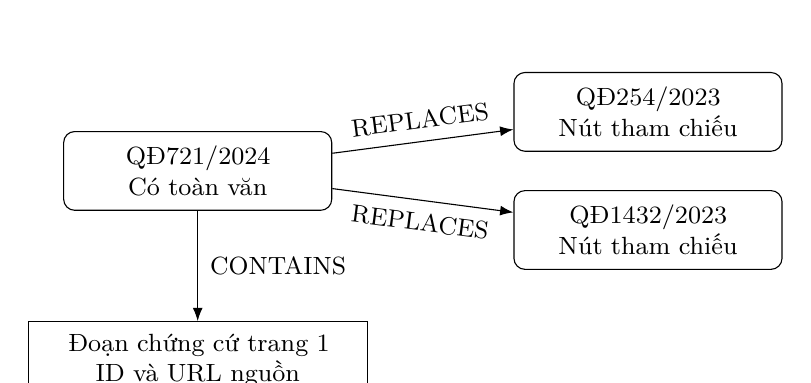
\begin{tikzpicture}[node distance=1.2cm, every node/.style={font=\small}, doc/.style={draw,rounded corners,align=center,text width=3.1cm,minimum height=1cm}, >=Latex]
\node[doc] (a) {QĐ721/2024\\Có toàn văn};
\node[doc, right=2.3cm of a,yshift=.75cm] (b) {QĐ254/2023\\Nút tham chiếu};
\node[doc, right=2.3cm of a,yshift=-.75cm] (c) {QĐ1432/2023\\Nút tham chiếu};
\node[draw,align=center,below=1.4cm of a,text width=4cm] (e) {Đoạn chứng cứ trang 1\\ID và URL nguồn};
\draw[->] (a)--node[above,sloped]{REPLACES}(b);
\draw[->] (a)--node[below,sloped]{REPLACES}(c);
\draw[->] (a)--node[right]{CONTAINS}(e);
\end{tikzpicture}
\caption{Ví dụ quan hệ theo QĐ721, không suy diễn toàn văn của nút tham chiếu.}
\end{figure}

QĐ721 ghi thay thế hai quyết định trên \cite{qd721}; chưa xác nhận đây là bản mới nhất. Tập 22 quan hệ chưa bao phủ mọi quan hệ trong corpus. Tham chiếu chưa rà không tự chuyển thành cạnh pháp lý.

\section{Thiết kế và kiểm chứng hệ thống}
\subsection{Luồng xử lý chung}
Hai phương pháp dùng chung corpus, encoder và bộ sinh. Khác biệt chính nằm ở cách tạo và xếp hạng tập chứng cứ. API FastAPI phục vụ giao diện React và trả cả đáp án, nguồn, trace, token và thời gian. Chế độ chỉ truy xuất cho phép kiểm tra đoạn được chọn mà không gọi Gemini. Cách tách này giúp nghiên cứu lỗi từng tầng mà không tiêu tốn thêm quota khi chỉ cần đánh giá tìm kiếm.

\begin{figure}[H]
\centering
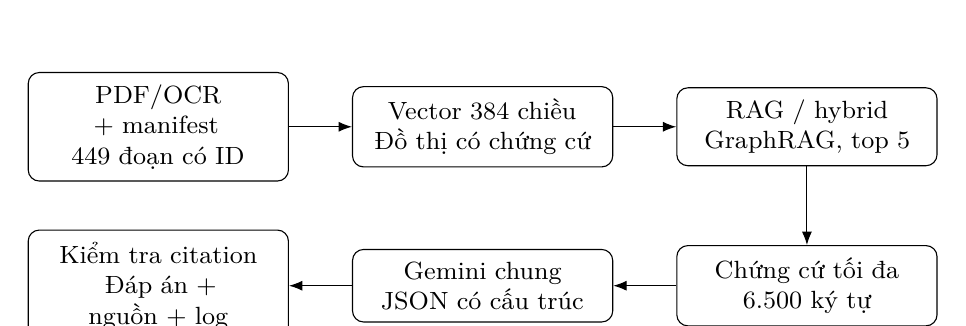
\begin{tikzpicture}[>=Latex, node distance=.7cm, every node/.style={font=\small}, box/.style={draw,rounded corners,align=center,minimum height=.85cm,text width=3cm}]
\node[box] (data) {PDF/OCR + manifest\\449 đoạn có ID};
\node[box,right=.8cm of data] (index) {Vector 384 chiều\\Đồ thị có chứng cứ};
\node[box,right=.8cm of index] (search) {RAG / hybrid\\GraphRAG, top 5};
\node[box,below=1cm of search] (context) {Chứng cứ tối đa\\6.500 ký tự};
\node[box,left=.8cm of context] (gen) {Gemini chung\\JSON có cấu trúc};
\node[box,left=.8cm of gen] (out) {Kiểm tra citation\\Đáp án + nguồn + log};
\draw[->] (data)--(index); \draw[->] (index)--(search);
\draw[->] (search)--(context); \draw[->] (context)--(gen); \draw[->] (gen)--(out);
\end{tikzpicture}
\caption{Luồng nguyên mẫu dùng cho thực nghiệm, với đầu ra truy vết.}
\end{figure}

\subsection{Embedding đoạn dài và nhất quán chỉ mục}
Trước sửa lỗi, 160/449 đoạn vượt cửa sổ encoder và có nguy cơ bị bỏ phần cuối. Cách mới chia thành cửa sổ tối đa 256 token với 64 token chồng lấp. Mỗi cửa sổ được mean pooling có mặt nạ, chuẩn hóa; các vector cửa sổ của cùng đoạn được trung bình rồi chuẩn hóa lại. Công thức khái quát với $W_d$ cửa sổ là:
\begin{equation}
 \mathbf e_d=\operatorname{norm}\!\left(\frac{1}{W_d}\sum_{w=1}^{W_d}\operatorname{norm}(\operatorname{pool}(d_w))\right).
\end{equation}
Đây là quy tắc tổng hợp của dự án, không phải bằng chứng rằng thông tin dài được hiểu hoàn hảo. Lợi ích kiểm chứng được là không bỏ âm thầm đuôi đoạn; ID và gold không thay đổi. Mọi phương pháp dùng cùng quy tắc, nên không đưa một phương pháp vào điều kiện embedding thuận lợi hơn.

Chỉ mục được dựng trong thư mục phiên bản riêng, kiểm tra đủ corpus, vector và đồ thị rồi mới chuyển liên kết \code{current} bằng thao tác atomic. Searcher giữ một phiên bản khi đọc. Nếu OCR hoặc embedding lỗi, bản đang dùng vẫn được giữ. Health kiểm tra artifact, hash và cấu hình encoder; chỉ mục không hợp lệ dẫn tới trạng thái chưa sẵn sàng và HTTP503, thay vì trả ``ready'' rồi lỗi khi chat.

\subsection{Ba chiến lược truy xuất}
RAG vector mã hóa câu hỏi và lấy 5 đoạn cosine cao nhất trên toàn corpus. Hybrid không graph lấy 5 đoạn cao nhất theo $s_h$ trên cùng corpus, không mở rộng cạnh và không thêm điểm thưởng. GraphRAG thực hiện các bước sau:
\begin{enumerate}
\item Lấy 3 hạt giống TF-IDF và 2 hạt giống vector, loại trùng.
\item Bổ sung đoạn theo chủ đề khớp và các đoạn kề hạt giống qua NEXT.
\item Đi tối đa hai bước qua các quan hệ văn bản, xét cả hai chiều khi mở rộng; thêm tối đa 3 đoạn có điểm hybrid cao của mỗi văn bản liên quan có toàn văn.
\item Nhận diện số hiệu/năm từ metadata và ý định hỏi quan hệ; bổ sung đoạn chứng cứ của cạnh đã được kiểm tra, cộng 0,7 điểm cho các đoạn này.
\item Xếp hạng ứng viên, chọn top 5, lưu trace và áp dụng cùng trần chứng cứ.
\end{enumerate}
Điểm thưởng và tập ứng viên là một phần của phương pháp được đánh giá. Vì vậy, khác biệt với RAG vector đo cả gói chiến lược. Đối chứng hybrid giúp kiểm tra tín hiệu từ vựng, nhưng chưa tách riêng hiệu ứng của mở rộng cạnh, chủ đề, NEXT và điểm thưởng. Nhận diện số hiệu dựa trên metadata của mọi văn bản, không cài riêng theo ID câu hỏi của bộ test.

\subsection{Sinh đáp án, từ chối và pacing}
Gemini trả JSON gồm trạng thái, đáp án và danh sách ID nguồn. Nhánh trả lời yêu cầu citation có thật và khớp danh sách; nhánh thiếu chứng cứ chỉ chấp nhận câu chuẩn ``Chưa xác định được từ tập tài liệu.''. Các nhóm citation như \code{[ID1, ID2]} được kiểm tra từng ID. Validation cấu trúc không chấm độ đúng ngữ nghĩa, nên các phát biểu sai phạm vi vẫn phải được đánh giá nội dung.

Model dùng trong lần đo là \code{gemini-3.5-flash-lite} \cite{gemini}. Cấu hình chung: temperature bằng 0, tối đa 2.048 token đầu ra, timeout 30 giây và một yêu cầu SDK cho mỗi lượt, không tự retry. Bộ điều phối trên cùng máy giữ khoảng cách ít nhất 5 giây giữa các request API/CLI bằng khóa tệp. Đây là nhịp khoảng 12 RPM; hạn mức 15 RPM do người dùng cung cấp chưa được coi là quota chung, vì Google quy định theo project, model và tier \cite{quota}.

\subsection{Kiểm chứng trước phép đo}
Đã hoàn tất 15 test hồi quy, compile Python, build TypeScript/Vite và HTTP smoke cho health/chat. Các test gồm sai phiên bản checkpoint, lỗi dựng chỉ mục, đoạn dài khác đuôi, từ chối kèm khẳng định, ID giả trong citation nhóm và các mode truy xuất. Test mô phỏng lỗi dịch vụ không gọi Gemini thật. Một lượt sinh HTTP kiểm tra sau sửa parser được lưu riêng và loại khỏi 40 lượt nghiên cứu chính. Kiểm tra bố cục giao diện bằng trình duyệt chưa thực hiện trong phiên review; không dùng build thành công để khẳng định đã kiểm tra đầy đủ giao diện.

\section{Thiết kế phép so sánh}
\subsection{Bộ câu hỏi và đơn vị quan sát}
Ba bộ được chạy ở tầng truy xuất. Bộ 30 câu ban đầu có 25 câu có gold, gồm 12 một điều, 8 nhiều điều và 5 phiên bản; 5 câu không có thông tin không được tính Recall. Bộ 8 câu quan hệ yêu cầu nối chứng cứ giữa văn bản hoặc trang. Bộ 20 dùng cho sinh chọn trước đáp án mới, mỗi nhóm có 4 câu: một điều, nhiều điều, phiên bản, quan hệ và ngoài corpus.

\begin{table}[H]
\centering\small
\caption{Quy mô thực nghiệm và mẫu số đánh giá}
\begin{tabularx}{\textwidth}{X r r X}
\toprule Bộ & Câu & Có gold & Phép đo\\
\midrule
30 câu nguyên trạng & 30 & 25 & Ba phương pháp truy xuất: 90 lượt.\\
8 câu quan hệ & 8 & 8 & Ba phương pháp truy xuất: 24 lượt.\\
20 câu có phạm vi rõ & 20 & 16 & Ba truy xuất: 60 lượt; hai sinh: 40 request.\\
\bottomrule
\end{tabularx}
\end{table}

Tổng 174 lượt truy xuất là $(30+8+20)\times3$, không phải 174 câu khác nhau. Bộ 20 kế thừa câu trong hai bộ trước; tám câu S/M thêm phạm vi ``bản hợp nhất QĐ744/2021 và QĐ666/2023''. Đây là thay đổi wording để giảm mơ hồ, không tạo một tập độc lập. Không cộng ba bộ rồi báo cáo như một mẫu độc lập lớn hơn.

\subsection{Phân tầng theo yêu cầu chứng cứ}
Câu một điều kiểm tra khả năng xác định một quy định cụ thể. Câu nhiều điều cần phối hợp ít nhất hai ý hoặc điều khoản. Câu phiên bản yêu cầu xác định đúng văn bản, giới hạn thời gian hoặc điều thay thế. Câu quan hệ kiểm tra các phát biểu sửa đổi, viện dẫn, thay thế giữa văn bản. Câu ngoài corpus kiểm tra việc từ chối trả lời học phí tương lai, lịch/hồ sơ cá nhân hoặc chương trình không có chứng cứ trong tập thu thập.

Phân tầng trước khi phân tích giúp tránh việc trung bình chung che khuất lỗi. Ví dụ, một phương pháp có thể tốt ở quan hệ nhưng kém hơn ở câu một điều; nếu bộ test chứa nhiều câu quan hệ thì mức tăng trung bình sẽ lớn. Bộ 20 cân bằng năm nhóm để thuận tiện đối chiếu, nhưng chưa phản ánh phân bố câu hỏi thực tế của sinh viên.

\subsection{Gold và nguy cơ thiên lệch}
Gold là đáp án và ID chứng cứ nội bộ đã đóng băng. Các câu quan hệ được viết sau khi xây đồ thị, nên có thể thuận lợi cho các cạnh đã biết. Chưa có người độc lập soạn câu, duyệt gold hoặc chấm đáp án. Gold S02 đòi hỏi học phí và điều kiện rút dù câu hỏi hỏi tuần; V05 chỉ yêu cầu tuần. Hai hệ thống được chấm cùng gold ở từng câu, nhưng sự không đồng nhất này ảnh hưởng cách hiểu độ đầy đủ và phải sửa trong bộ mới, không sửa ngược để tăng điểm hiện tại.

\subsection{Biến được giữ chung và biến thay đổi}
\begin{table}[H]
\centering\small
\caption{Điều kiện kiểm soát của phép so sánh}
\begin{tabularx}{\textwidth}{l X}
\toprule Thành phần & Thiết lập\\
\midrule
Corpus và ID & Cùng 449 đoạn, hash và phiên bản chỉ mục.\\
Embedding & Cùng MiniLM đa ngôn ngữ, revision và pooling cửa sổ.\\
Truy xuất đầu ra & Top 5; cùng trần 6.500 ký tự chứng cứ cho bộ sinh.\\
Model sinh & Gemini 3.5 Flash-Lite, cùng prompt và JSON schema.\\
Sinh và dịch vụ & Temperature 0; 2.048 token; timeout 30 giây; không retry.\\
Thứ tự gọi & Đảo RAG/GraphRAG luân phiên theo câu.\\
Thứ tự truy xuất & Xoay thứ tự ba phương pháp theo câu, warm encoder trước đo.\\
Biến thay đổi & Tập ứng viên, tín hiệu xếp hạng, mở rộng đồ thị và điểm thưởng.\\
\bottomrule
\end{tabularx}
\end{table}

Giới hạn ký tự chung không làm số token thực tế bằng nhau: hai phương pháp lấy nội dung khác nhau và tạo đáp án dài khác nhau. Top 5 chung cũng chưa kiểm soát độ bao phủ khi gold trải trên nhiều đoạn. Vì vậy, đây là so sánh hai pipeline trong cùng ngân sách cấu hình, không phải phép đo chỉ một biến ``có đồ thị''.

\subsection{Quy trình đo và lưu vết}
Trước đo, corpus, vector, graph, cấu hình và runtime được ghi fingerprint. Snapshot câu hỏi được lưu cùng run; checkpoint bị chặn nếu cấu hình hiệu dụng hoặc model thay đổi. Đánh giá truy xuất ghi danh sách gold, ID trả về, Recall, độ trễ và trace. Đánh giá sinh ghi JSON thô, lỗi, model/provider, token, thời điểm request, thời gian chờ pacing và thời gian pipeline. Các artifact cũ được giữ nguyên.

Có 40 request thật cho 20 cặp, không lỗi dịch vụ hoặc quota trong run. R03/GraphRAG ban đầu bị validator chặn vì nhóm citation hai ID. Sau sửa parser, toàn bộ JSON thô đã lưu được kiểm tra lại offline: 20/20 cặp hợp lệ, không sửa đáp án thô, không gọi API mới. Artifact dẫn xuất ghi hash log gốc và validator. Token và thời gian vẫn lấy request gốc; không mô tả sự kiện này như một đợt gọi lại model sau sửa.

\subsection{Điều kiện thời gian và môi trường}
Runtime ghi nhận Python 3.13.9, Torch 2.6.0, NumPy 2.2.6, scikit-learn 1.7.2, NetworkX 3.4.2 và google-genai 2.10.0. Chỉ mục dựng khoảng 28,80 giây, không bao gồm tạo OCR thủ công hoặc tải encoder lần đầu. Truy xuất chạy trên CPU; phép đo truy xuất diễn ra khi tiến trình đánh giá Gemini cũng hoạt động, có outlier. Nghiên cứu không kiểm tra nhiều người dùng đồng thời, không khảo sát tải hay độ ổn định qua nhiều ngày. Một lần đo chỉ hỗ trợ mô tả run này.

\subsection{Chỉ số truy xuất và đáp án}
Với câu $i$, gọi $G_i$ là tập gold và $R_i^5$ là top 5. Recall được tính:
\begin{equation}
 \mathrm{Recall@5}_i=\frac{|G_i\cap R_i^5|}{|G_i|},\qquad
 \overline{\mathrm{Recall@5}}=\frac{1}{N_g}\sum_{i:|G_i|>0}\mathrm{Recall@5}_i.
\end{equation}
Mỗi câu có trọng số như nhau, không phải trung bình gộp mọi gold. All-gold là số câu có $G_i\subseteq R_i^5$. Hai chỉ số khác nhau: tăng số gold ở câu trước đây thiếu nhiều có thể làm Recall tăng dù số câu tìm đủ giảm. Câu không có gold được loại khỏi mẫu số, không đặt Recall bằng 0 hoặc 1.

\begin{table}[H]
\centering\small
\caption{Rubric nhị phân dùng chấm sơ bộ 40 đáp án}
\begin{tabularx}{\textwidth}{l X}
\toprule Chỉ số & Điều kiện đạt\\
\midrule
Đúng ý chính & Đúng thông tin được hỏi và đúng phạm vi văn bản; trả sai trọng tâm hoặc từ chối sai là 0.\\
Đủ ý & Bao phủ các ý, điều kiện, ngoại lệ mà gold của câu yêu cầu.\\
Nguồn hỗ trợ & Những phát biểu đã trả được citation hỗ trợ và đúng phạm vi; có thể đạt dù đáp án thiếu ý.\\
Từ chối phù hợp & Chỉ áp dụng câu ngoài corpus; từ chối chuẩn, không thêm khẳng định ngoài chứng cứ.\\
\bottomrule
\end{tabularx}
\end{table}

Trợ lý AI đối chiếu từng đáp án với gold và chứng cứ, ghi chú lý do. Đây không phải kết quả chấm người hoặc một bộ chấm đã được kiểm định. Không dùng dò từ khóa để thay thế đọc nội dung. Nguồn hỗ trợ và đúng ý chính được tách riêng: câu M02 có thể dẫn đúng nguồn của 33 tín chỉ nhưng chưa trả mức khối lượng cuối cùng 27 tín chỉ trong gold. Mẫu số nội dung là 16 câu trả lời được, còn mẫu số từ chối là 4 câu ngoài corpus.

\subsection{Độ trễ, token và so sánh cặp}
Độ trễ pipeline đo sau khi encoder/index đã nạp, loại thời gian chờ pacing; \code{wall_ms} và \code{pacing_wait_ms} được lưu riêng. Trung vị hỗ trợ đọc dữ liệu khi có outlier, còn trung bình phản ánh các giá trị của run. Token vào/ra lấy từ phản hồi API, cộng trên 20 lượt của mỗi phương pháp. Không ước tính tiền hoặc tuyên bố tốc độ ổn định chỉ từ lần chạy này.

Với điểm đúng ý chính, mỗi câu ghép RAG và GraphRAG thành một cặp. Kiểm định McNemar exact tương đương nhị thức hai phía trên các cặp bất đồng. Nếu $b=5$ cặp GraphRAG đúng hơn và $c=2$ cặp RAG đúng hơn, xác suất tham khảo là:
\begin{equation}
 p=2\sum_{j=0}^{2}\binom{7}{j}(0{,}5)^7=0{,}453125.
\end{equation}
Phép tính chỉ mang tính thăm dò. Bộ câu không lấy mẫu ngẫu nhiên độc lập; giá trị $p$ không loại bỏ thiên lệch và không chứng minh hai phương pháp tương đương. Độ lớn hiệu ứng và phân tích trường hợp được đọc cùng hạn chế mẫu.

\section{Kết quả thực nghiệm}
\subsection{Chất lượng truy xuất trên ba bộ}
\begin{table}[H]
\centering\small
\caption{Recall@5 và số câu tìm đủ mọi gold, sau sửa lỗi}
\begin{tabular}{llrrr}
\toprule Bộ & Phương pháp & Có gold & Recall@5 & All-gold\\
\midrule
30 câu & RAG vector & 25 & 0,7400 & 17/25\\
 & Hybrid & 25 & 0,7200 & 15/25\\
 & GraphRAG & 25 & 0,7800 & 16/25\\
\midrule
8 quan hệ & RAG vector & 8 & 0,2500 & 1/8\\
 & Hybrid & 8 & 0,6250 & 5/8\\
 & GraphRAG & 8 & 1,0000 & 8/8\\
\midrule
20 câu & RAG vector & 16 & 0,6250 & 8/16\\
 & Hybrid & 16 & 0,5938 & 8/16\\
 & GraphRAG & 16 & 0,7813 & 11/16\\
\bottomrule
\end{tabular}
\end{table}
\sourcefile{evaluation/runs/research_20261001/retrieval_summary.csv}

\begin{figure}[H]
\centering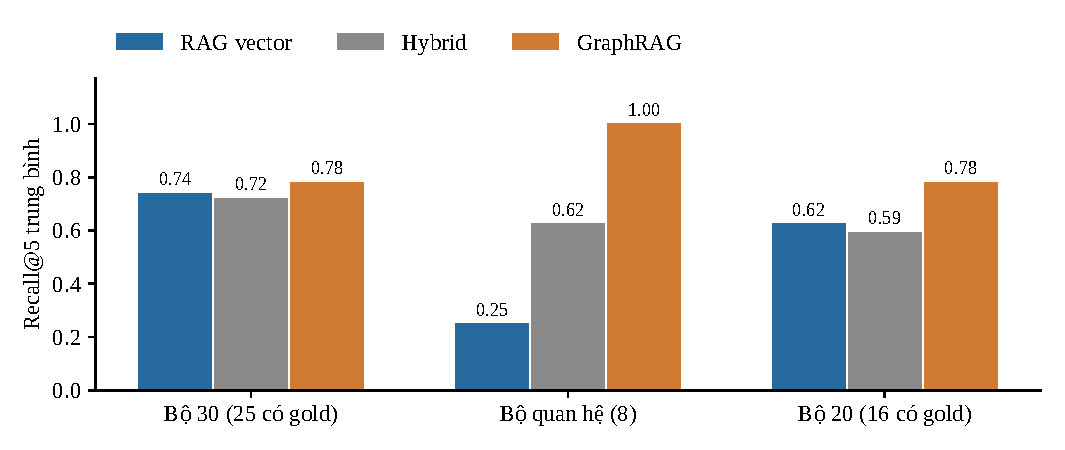
\includegraphics[width=\textwidth]{figures/recall_suites.pdf}
\caption{So sánh truy xuất; ba bộ có chồng lấp, không cộng thành mẫu độc lập.}
\end{figure}

Trên bộ 30, mức tăng Recall của GraphRAG so với RAG là 0,04, nhưng All-gold giảm một câu. Kết quả này cho thấy việc chọn một chỉ số duy nhất có thể dẫn đến kết luận thiếu cân bằng. Trên bộ quan hệ, hybrid đã tăng Recall 0,375 so với vector thuần; phần tăng thêm từ hybrid tới GraphRAG cũng là 0,375. Tín hiệu từ vựng vì vậy có đóng góp quan sát được trước khi xét đồ thị.

Trên bộ 20 có phạm vi rõ, GraphRAG tìm đủ gold ở 11/16 câu, hai đối chứng đạt 8/16. Chênh lệch với bộ 30 không thể được coi là tác động riêng của sửa code: phân bố nhóm và câu chữ đều khác. Bộ quan hệ có lợi thế thiết kế cho các cạnh đã xây; Recall bằng 1 ở đây là kết quả trên tám câu nội bộ, chưa là ước lượng cho mọi câu hỏi quan hệ mới.

\subsection{Phân nhóm và chất lượng đáp án}
\begin{figure}[H]
\centering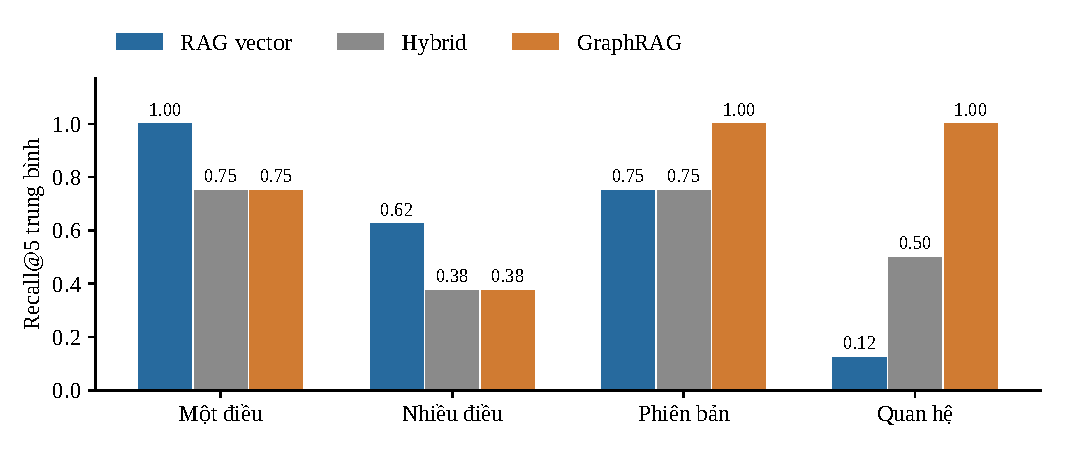
\includegraphics[width=\textwidth]{figures/recall_groups.pdf}
\caption{Recall@5 của bộ 20: mỗi nhóm trong hình có bốn câu có gold.}
\end{figure}

Nhóm một điều: RAG đạt 1,00, hybrid và GraphRAG cùng 0,75. Nhóm nhiều điều: RAG 0,625, hai phương pháp còn lại 0,375. Nhóm phiên bản: GraphRAG 1,00, hai đối chứng 0,75. Nhóm quan hệ: RAG 0,125, hybrid 0,50, GraphRAG 1,00. Đồ thị không tự bảo đảm cải thiện khi nhiều điều kiện nằm trong một văn bản; cạnh tranh top 5 và chọn phạm vi vẫn có thể làm mất chứng cứ.

\begin{table}[H]
\centering\small
\caption{Đánh giá nội dung sơ bộ bằng trợ lý AI, chưa chấm người độc lập}
\begin{tabular}{lcc}
\toprule Chỉ số & RAG vector & GraphRAG\\
\midrule
Đúng ý chính/phạm vi & 8/16 (50,00\%) & 11/16 (68,75\%)\\
Đủ ý theo gold & 4/16 (25,00\%) & 8/16 (50,00\%)\\
Nguồn hỗ trợ phát biểu & 9/16 (56,25\%) & 12/16 (75,00\%)\\
Từ chối phù hợp ngoài corpus & 4/4 & 4/4\\
\bottomrule
\end{tabular}
\end{table}
\sourcefile{evaluation/runs/research_20261001/answer_scores.json}

\begin{table}[H]
\centering\small
\caption{Số câu đạt đúng/đủ/nguồn trong từng nhóm, mẫu số mỗi ô là 4}
\begin{tabular}{lcc}
\toprule Nhóm & RAG & GraphRAG\\
\midrule
Một điều & 4 / 2 / 4 & 3 / 1 / 3\\
Nhiều điều & 1 / 0 / 2 & 0 / 0 / 1\\
Phiên bản & 3 / 2 / 3 & 4 / 3 / 4\\
Quan hệ & 0 / 0 / 0 & 4 / 4 / 4\\
\bottomrule
\end{tabular}
\end{table}

Mức tăng 3 câu đúng của GraphRAG tương ứng 18,75 điểm phần trăm trên 16 câu. Có 5 cặp GraphRAG thắng, 2 cặp RAG thắng và 9 cặp bằng nhau. Lợi ích tập trung ở 4 câu quan hệ và V02; bất lợi nằm ở S07 và M01. Với $p=0{,}4531$, chưa đủ bằng chứng ở mức 0,05 về ưu thế chung. Cả hai xử lý phù hợp bốn câu ngoài corpus, nhưng mẫu này chưa bao gồm toàn bộ kiểu yêu cầu thiếu chứng cứ.

\subsection{Độ trễ và lượng token}
\begin{table}[H]
\centering\small
\caption{Chi phí quan sát trên 20 lượt sinh của mỗi phương pháp}
\begin{tabular}{lrr}
\toprule Chỉ số & RAG vector & GraphRAG\\
\midrule
Độ trễ trung bình pipeline (ms) & 1.636,32 & 1.747,54\\
Độ trễ trung vị pipeline (ms) & 1.486,55 & 1.709,29\\
Token vào tổng & 29.484 & 31.723\\
Token ra tổng & 1.735 & 2.549\\
Token tổng & 31.219 & 34.272\\
\bottomrule
\end{tabular}
\end{table}
\sourcefile{evaluation/runs/research_20261001/generation_revalidated.json}

\begin{figure}[H]
\centering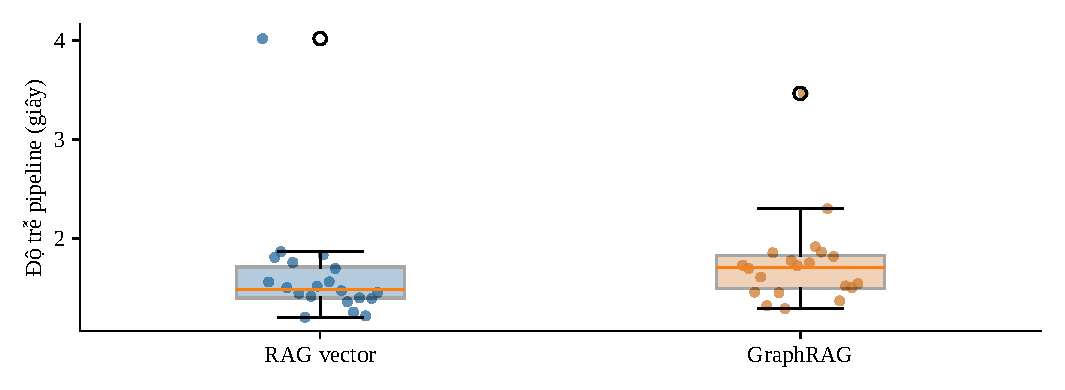
\includegraphics[width=\textwidth]{figures/latency.pdf}
\caption{Phân bố 20 độ trễ mỗi phương pháp; loại thời gian chờ pacing.}
\end{figure}

GraphRAG tăng khoảng 111,22 ms trung bình, tương đương 6,8\% so với RAG trong run này. Tổng token tăng 3.053, khoảng 9,8\%; token đầu ra tăng vì có thêm câu trả lời và nội dung dài hơn. RAG từ chối sai 7/16 câu có đáp án, GraphRAG từ chối sai 3/16. Vì thế, token thấp hơn của RAG một phần gắn với việc không trả lời câu có thể trả lời; chưa thể coi đó là ưu thế hiệu quả độc lập với chất lượng.

Độ trễ truy xuất trung vị trên bộ 30 lần lượt là 9,705 ms, 11,895 ms và 13,480 ms cho RAG, hybrid và GraphRAG. Trung bình tương ứng là 49,872 ms, 31,522 ms và 14,127 ms. Sự đảo thứ tự giữa trung bình và trung vị thể hiện ảnh hưởng của outlier trong điều kiện có tiến trình khác hoạt động. Không sử dụng các trung bình này để khẳng định GraphRAG luôn nhanh hơn truy xuất vector.

Khoảng cách nhỏ nhất giữa thời điểm bắt đầu 40 request là 5,000067 giây, phù hợp nhịp đã cấu hình. Chờ pacing và thời gian nạp model không nằm trong độ trễ bảng. Người dùng thực tế có thể chờ lâu hơn độ trễ pipeline nếu phải xếp hàng. Nghiên cứu không quy đổi token sang tiền, không đo thông lượng tải lớn và không suy ra thời gian phục vụ nhiều người dùng từ số đo đơn lẻ.

\section{Phân tích nguyên nhân và độ tin cậy}
\subsection{Trường hợp GraphRAG hỗ trợ tốt hơn}
\textbf{V02 --- xác định văn bản bị thay thế.} Câu hỏi yêu cầu quyết định được quy chế hợp nhất thay thế. RAG không lấy được khoản 2 Điều 22 và từ chối. GraphRAG đưa vào đúng chứng cứ, trả QĐ787/2018 cùng ngày 09/08/2018. Điểm cải thiện nằm ở việc tìm phát biểu quan hệ trong phần hiệu lực/thi hành, vốn có thể kém tương đồng với câu hỏi so với đoạn nội dung đào tạo.

\textbf{R01 --- hai văn bản bị QĐ721 thay thế.} GraphRAG nhận diện số hiệu và ý định thay thế, ưu tiên đoạn chứng cứ trang 1. Đáp án nêu QĐ254/2023 và QĐ1432/2023; RAG thiếu đoạn và từ chối. Hai đích là nút tham chiếu, nhưng câu trả lời vẫn có chứng cứ vì phát biểu thay thế nằm trong QĐ721. Hệ thống không cần giả định toàn văn của các nút đích để trả câu hỏi này. Lỗi dấu gạch OCR trong ký hiệu được ghi chú, không làm thay đổi số hiệu trong tiêu chí chấm.

\textbf{R02 --- căn cứ nằm ở hai trang.} Quy định khóa luận dẫn TT08/2021 và QĐ239/2022. GraphRAG tìm đủ chứng cứ trang 1 và 2; RAG chỉ tìm được một phần và từ chối. Trường hợp này cho thấy cần đánh giá chuỗi chứng cứ, thay vì chỉ kiểm tra có nhắc đúng tên văn bản hay không. Một câu trả lời đầy đủ phải hỗ trợ cả hai ý, không dùng một citation để bao trùm phát biểu không nằm trong đoạn đó.

\textbf{R03 và R06 --- quan hệ nối giữa văn bản.} R03 yêu cầu QĐ663 sửa QĐ787 \cite{qd663} và quan hệ của bản hợp nhất với QĐ663; R06 yêu cầu hai quyết định bị TT08 thay thế. GraphRAG trả đủ, RAG từ chối do thiếu chứng cứ. R03 cũng phát hiện lỗi kỹ thuật đọc citation nhóm. Tách lỗi validator khỏi lỗi nội dung giúp tránh chấm một đáp án có hai ID hợp lệ thành thất bại của mô hình; việc kiểm tra lại offline được ghi rõ trong hồ sơ.

\subsection{Vì sao có lợi ích ở nhóm này?}
Số hiệu/năm là tín hiệu từ vựng mạnh; quan hệ sửa đổi hoặc thay thế là thông tin có cấu trúc. GraphRAG kết hợp các tín hiệu này với cạnh đã có câu dẫn, đưa đoạn chứng cứ vào ứng viên và cộng điểm ưu tiên. Trace và đoạn trả về phù hợp với cơ chế này. Tuy vậy, đây là giải thích từ triển khai và quan sát, chưa phải kết luận nhân quả riêng cho đồ thị.

Hybrid cải thiện đáng kể trên bộ 8 quan hệ, từ 0,25 lên 0,625. Phần chênh lệch còn lại với GraphRAG có thể liên quan đồng thời đến cạnh, mở rộng ứng viên và điểm thưởng. Để cô lập nguyên nhân cần các ablation giữ nguyên phần còn lại, chẳng hạn bỏ điểm thưởng hoặc bỏ cạnh trong cùng cơ chế ứng viên. Các ablation này là đề xuất, chưa được chạy và không có số liệu trong báo cáo.

\subsection{Trường hợp RAG tốt hơn và lỗi chung}
\textbf{S07 --- dẫn nguồn tồn tại nhưng sai phạm vi.} Câu hỏi đã nêu bản hợp nhất và hỏi khoảng điểm A/F. RAG lấy khoản 7 Điều 9, trả A từ 8,5 đến 10 và F dưới 4. GraphRAG đưa vào TT08 và trả A bằng 4, F bằng 0, tức giá trị quy đổi thay vì khoảng điểm. Citation không giả, nhưng phát biểu không đáp ứng phạm vi và trọng tâm câu hỏi. Đây là bằng chứng rằng kiểm tra ID hợp lệ không thay thế kiểm tra ý nghĩa.

Nguyên nhân quan sát được gồm việc nhiều văn bản cùng chứa từ khóa điểm A/F và xếp hạng chưa bảo đảm chứng cứ thuộc văn bản được hỏi. Việc thêm số hiệu vào câu có thể nâng đoạn mở đầu hoặc đoạn quan hệ, cạnh tranh chỗ với nội dung điều khoản trong top 5. Cần kiểm tra trace và cơ chế giới hạn phạm vi, thay vì cài câu trả lời riêng cho S07. Một giải pháp có thể là dùng metadata để ưu tiên phạm vi rõ, nhưng phải đánh giá lại trên bộ độc lập trước khi kết luận hiệu quả.

\textbf{M01 --- RAG trả một phần, GraphRAG từ chối.} RAG trả GPA tối thiểu 2,00 và thời hạn cấp bằng ba tháng sau khi đủ điều kiện/nghĩa vụ, đạt ý chính nhưng thiếu các điều kiện khác trong gold. GraphRAG không tìm đủ hai chứng cứ và từ chối. Chỉ tăng liên kết đồ thị không bảo đảm tìm đầy đủ các điều kiện trong cùng văn bản. Câu này đồng thời cho thấy điểm đúng và điểm đủ phải được tách.

\textbf{M02 --- con số có nguồn nhưng chưa phải mức cuối cùng.} Cả hai lấy khoản 3 Điều 7 về 33 tín chỉ trong đợt đăng ký chính, bỏ lỡ khoản 5 về mức 27 của khối lượng học kỳ cùng nghĩa vụ điều chỉnh. Thông tin tuần rút 03--08 đúng nhưng thiếu ý học phí theo gold. Không nên gọi 33 là số bịa: nó có trong chứng cứ, song chưa trả đúng giới hạn mà câu hỏi và gold yêu cầu. Lỗi nằm ở phối hợp quy định và nhận diện giai đoạn áp dụng.

\textbf{M05/M08 --- thiếu một phần chứng cứ dẫn tới từ chối sai.} M05 bỏ lỡ nội dung công nhận/chuyển đổi 50\%; M08 tìm được tỷ lệ trực tuyến 30\% nhưng thiếu đoạn ít nhất hai điểm thành phần. Cả hai từ chối trên câu có đáp án trong corpus. Với ngân sách top 5, đoạn gần nghĩa có thể chiếm chỗ các điều kiện cần thiết. Việc trả lời thận trọng giúp tránh suy diễn, nhưng không xóa lỗi truy xuất khiến hệ thống mất khả năng trả lời.

\subsection{Thiếu ý dù đã có đoạn đúng}
S02 trả đúng tuần rút nhưng bỏ điều kiện và học phí trong gold; S04 trả đúng 30\% nhưng bỏ ngoại lệ bất khả kháng theo hướng dẫn; V01 trả đúng sáu năm nhưng thiếu ngoại lệ. Những lỗi này xuất hiện sau khi đã tìm được đoạn liên quan, nên chỉ nâng Recall chưa đủ. Prompt hoặc bộ kiểm tra điều kiện có thể hỗ trợ, nhưng cần cân bằng độ dài và tránh ép mô hình thêm nội dung không được nguồn hỗ trợ. Ngược lại, S06 và V04 đều trả đủ ở cả hai phương pháp, minh họa trường hợp GraphRAG không tạo thêm lợi ích nội dung.

\subsection{Các đe dọa đến độ tin cậy}
\textbf{Tính đại diện của bộ câu.} Bộ 20 được chọn cân bằng để phân tích, không lấy từ phân bố truy vấn thực. Bộ 8 quan hệ được soạn sau đồ thị, có khả năng đo đúng những quan hệ đã được ưu tiên. Các câu trong ba bộ chồng lấp; tăng số lượt chạy không làm tăng tương ứng độ đa dạng mẫu. Kết quả được diễn giải trong phạm vi nội bộ, không suy rộng thành độ chính xác cho sinh viên HaUI nói chung.

\textbf{Tính tin cậy của chấm điểm.} Trợ lý AI vừa hỗ trợ phát triển vừa chấm sơ bộ; chưa có chấm mù, hai người chấm hoặc độ đồng thuận. Gold có yêu cầu độ đầy đủ chưa thống nhất giữa S02 và V05. Dù hai phương pháp dùng cùng rubric theo từng câu, thiên lệch đánh giá vẫn có thể tồn tại. Người thực hiện cần đọc lại đáp án, trang PDF và ghi chú trước khi dùng bảng như kết quả chính thức cuối cùng.

\textbf{Tính cô lập của biến.} GraphRAG khác vector thuần ở từ vựng, ứng viên, mở rộng và điểm thưởng. Hybrid chỉ kiểm soát một phần từ vựng. Trọng số 0,55/0,45, điểm thưởng 0,7 và top 5 chưa được lựa chọn trên tập phát triển tách biệt. Không thể quy mọi mức tăng cho đồ thị hoặc coi cấu hình hiện tại đã tối ưu.

\textbf{Chất lượng dữ liệu và thời gian.} OCR chưa hiệu đính toàn bộ; các quan hệ được kiểm tra khớp câu dẫn trong trang/đoạn nhưng chưa phải rà pháp lý đầy đủ. Corpus chưa xác minh hiệu lực hiện hành và thiếu toàn văn 13 nút tham chiếu. Kết quả trả về phải được đọc theo văn bản đã có, không dùng cho kết luận quy chế mới nhất. Bộ nguồn cũng không đại diện mọi quy định của trường.

\textbf{Tái lập và dịch vụ ngoài.} Revision embedding, cấu hình, hash và log được lưu, giúp dựng lại quá trình. Tuy nhiên, Gemini là dịch vụ ngoài có thể thay đổi; temperature bằng 0 không bảo đảm đáp án tuyệt đối giống qua mọi lần gọi. Dependency trực tiếp được pin nhưng chưa khóa đầy đủ dependency gián tiếp hoặc kiểm tra cài mới sạch. Độ trễ chỉ có một run, chịu mạng, lịch CPU và phía provider; không suy ra khả năng tải lớn.

\subsection{Đợt đánh giá tiếp theo phù hợp quy mô đề tài}
Ưu tiên tiếp theo là chất lượng thiết kế thay vì tăng số request lớn: đóng băng corpus, nhờ người độc lập soạn khoảng 30 câu phân tầng, duyệt gold trực tiếp trên PDF và tách tập phát triển khỏi tập đánh giá. Có thể chấm mù hai phương pháp theo rubric thống nhất, ghi bất đồng và cách phân xử. Các câu mới nên bao gồm điều kiện/ngoại lệ, số hiệu viết khác nhau, phạm vi văn bản rõ và yêu cầu ngoài corpus.

Một đợt ablation nhỏ có thể giữ chung điểm hybrid và ngân sách rồi lần lượt bỏ mở rộng pháp lý hoặc bỏ điểm thưởng. Chỉ khi có số liệu mới mới kết luận đóng góp riêng của từng thành phần. Mở rộng data nên xuất phát từ khoảng thiếu chứng cứ hoặc mục tiêu mới, kèm hiệu đính OCR và cập nhật gold; không thêm văn bản chỉ để tăng số trang hoặc độ lớn corpus. Những bước này chưa được thực hiện trong nghiên cứu hiện tại.

\section{Kết luận và hướng phát triển}
Nghiên cứu so sánh hai pipeline trên cùng corpus HaUI, có đối chứng hybrid và trace. Lỗi kỹ thuật được sửa trước đo, lỗi nội dung được giữ để phân tích.

GraphRAG có Recall@5 cao hơn trên từng bộ, nhưng All-gold bộ 30 là 16/25 so với 17/25 của RAG. Hybrid cho thấy đóng góp từ vựng; chưa cô lập hiệu ứng đồ thị.

Lợi ích tập trung ở phiên bản/quan hệ; RAG tốt hơn ở S07/M01. Câu nhiều điều là điểm yếu chung. Cần chọn phương pháp theo yêu cầu chứng cứ.

Điểm sơ bộ đúng là 8/16 và 11/16, đủ ý là 4/16 và 8/16; cả hai từ chối phù hợp 4/4. Citation có thật chưa ngăn sai phạm vi. Kiểm định cặp chưa cho bằng chứng đủ mạnh về ưu thế chung.

GraphRAG tăng khoảng 9,8\% token và 6,8\% độ trễ trung bình; RAG ít token hơn cùng với nhiều từ chối sai. Không suy ra hiệu năng tải lớn.

\subsection{Ưu tiên phát triển}
Ưu tiên là hiệu đính OCR, thống nhất gold, kiểm soát phạm vi bằng metadata và soạn tập độc lập có chấm mù. Ablation nhỏ cần tách cạnh với điểm thưởng. Các cải tiến phải được đo trên snapshot mới và giữ lịch sử cũ.

Kết luận giới hạn ở bộ nội bộ và lần đo 01/10/2026. GraphRAG có triển vọng cho quan hệ/phiên bản; độ đầy đủ và phạm vi vẫn cần cải thiện ở cả hai.

\clearpage
\addcontentsline{toc}{section}{Tài liệu tham khảo}
\begin{thebibliography}{99}
\small\setstretch{1.15}
\bibitem{lewis} P. Lewis và cộng sự, ``Retrieval-Augmented Generation for Knowledge-Intensive NLP Tasks,'' NeurIPS, 2020. \url{https://arxiv.org/abs/2005.11401}.
\bibitem{sbert} N. Reimers và I. Gurevych, ``Sentence-BERT: Sentence Embeddings using Siamese BERT-Networks,'' EMNLP-IJCNLP, 2019. \url{https://arxiv.org/abs/1908.10084}.
\bibitem{multilingual} N. Reimers và I. Gurevych, ``Making Monolingual Sentence Embeddings Multilingual using Knowledge Distillation,'' EMNLP, 2020. \url{https://arxiv.org/abs/2004.09813}.
\bibitem{edge} D. Edge và cộng sự, ``From Local to Global: A Graph RAG Approach to Query-Focused Summarization,'' arXiv:2404.16130, 2024; bản v2, 2025. \url{https://arxiv.org/abs/2404.16130}.
\bibitem{gemini} Google, ``Gemini 3.5 Flash-Lite,'' tài liệu Gemini API, truy cập 01/10/2026. \url{https://ai.google.dev/gemini-api/docs/models/gemini-3.5-flash-lite}.
\bibitem{quota} Google, ``Rate limits,'' tài liệu Gemini API, truy cập 01/10/2026. \url{https://ai.google.dev/gemini-api/docs/rate-limits}.
\bibitem{qc2023} Trường Đại học Công nghiệp Hà Nội, ``Quy chế đào tạo trình độ đại học, bản hợp nhất QĐ744/2021 và QĐ666/2023,'' PDF 28 trang trên SICT; thu thập 28/09/2026. \href{https://sict.haui.edu.vn/media/29/uffile-upload-no-title29811.pdf}{PDF chính thức trên SICT HaUI}.
\bibitem{qd721} Trường Đại học Công nghiệp Hà Nội, ``Quyết định 721/QĐ-ĐHCN ngày 03/06/2024 về quy định tổ chức đánh giá kết quả học tập,'' PDF 59 trang; thu thập 28/09/2026. \href{https://cps.haui.edu.vn/media/quyet-dinh-721-ngay-03-06-2024-ve-viec-ban-hanh-quy-dinh-to-chuc-dgkqht-cua-nguoi-hoc-truong-dhcn-hn\%20\%285\%29.pdf}{PDF chính thức trên CPS HaUI}.
\bibitem{qd663} Trường Đại học Công nghiệp Hà Nội, ``Quyết định 663/QĐ-ĐHCN ngày 12/07/2019 sửa đổi quy chế theo QĐ787/2018,'' PDF 6 trang; thu thập 28/09/2026. \href{https://dttc.haui.edu.vn/media/2/uftai-ve-tai-day2712.pdf}{PDF chính thức trên DTTC HaUI}.
\bibitem{artifacts} Dự án cá nhân RAG/GraphRAG HaUI, ``Hồ sơ thực nghiệm ngày 01/10/2026,'' corpus manifest, cấu hình, log API, bảng truy xuất và điểm sơ bộ. Bản cục bộ: \code{evaluation/runs/research_20261001/}; mô tả sửa lỗi: \code{docs/FIX_REPORT_2026-10-01.md}. Đây là dữ liệu dự án, chưa công bố như một bài báo độc lập.
\end{thebibliography}
\noindent\small URL của toàn bộ 9 nguồn được lưu trong \code{data/source_manifest.csv}. Các tài liệu HaUI được dùng theo nội dung đã thu thập, không mặc nhiên xác nhận hiệu lực hiện hành. Liên kết PDF hỗ trợ đối chiếu trang; hash của bản cục bộ giúp phát hiện thay đổi tệp.

\clearpage
\section*{PHỤ LỤC: ĐỐI CHIẾU CÂU HỎI VÀ TÁI LẬP}
\addcontentsline{toc}{section}{Phụ lục: Đối chiếu câu hỏi và tái lập}
\noindent Bảng ghi điểm đúng ý chính sơ bộ: 1 đạt, 0 chưa đạt; TC là từ chối phù hợp ngoài corpus. Câu đầy đủ, gold, đáp án nguyên bản và ghi chú nằm trong hồ sơ thực nghiệm \cite{artifacts}.
\begin{table}[H]
\centering\small\setstretch{1.05}\renewcommand{\arraystretch}{1.12}
\begin{tabularx}{\textwidth}{l X cc}
\toprule ID & Nội dung rút gọn & RAG & Graph \\
\midrule
S02 & Tuần rút lớp học phần & 1 & 1 \\
S04 & Tỷ lệ đào tạo trực tuyến & 1 & 1 \\
S06 & Thi bổ sung do lý do chính đáng & 1 & 1 \\
S07 & Khoảng điểm A và F & 1 & 0 \\
M01 & Điều kiện tốt nghiệp và thời hạn cấp bằng & 1 & 0 \\
M02 & Khối lượng tín chỉ và rút học phần & 0 & 0 \\
M05 & Học chương trình thứ hai, công nhận tín chỉ & 0 & 0 \\
M08 & Điểm thành phần và đánh giá trực tuyến & 0 & 0 \\
V01 & Thời gian tối đa của chương trình 4 năm & 1 & 1 \\
V02 & Văn bản bị quy chế hợp nhất thay thế & 0 & 1 \\
V04 & Thời gian học tối đa trong TT08 & 1 & 1 \\
V05 & Tuần rút theo quy chế hợp nhất & 1 & 1 \\
R01 & Hai quyết định bị QĐ721 thay thế & 0 & 1 \\
R02 & Căn cứ TT08 và QĐ239 của quy định khóa luận & 0 & 1 \\
R03 & Quan hệ QĐ663, QĐ787 và bản hợp nhất & 0 & 1 \\
R06 & Hai quyết định bị TT08 thay thế & 0 & 1 \\
U01 & Học phí năm 2026–2027 & TC & TC \\
U02 & Lịch thi cá nhân & TC & TC \\
U03 & Tình trạng tốt nghiệp cá nhân & TC & TC \\
U05 & Đào tạo sau đại học AI hiện tại & TC & TC \\
\bottomrule
\end{tabularx}
\end{table}

\subsection*{Artifact cần giữ}
\noindent\small
\code{retrieval.json} và CSV lưu 174 lượt truy xuất; \code{answer_scores.json} lưu rubric, người/chương trình chấm và ghi chú; \code{generation_revalidated.json} lưu kết quả kiểm tra lại dẫn xuất. Log API gốc là \code{evaluation/runs/gemini_research_20261001_35lite.jsonl}. Bộ 20 câu nằm ở \code{evaluation/questions_research_20261001.jsonl}. Hash dùng tạo hình/bảng của báo cáo nằm ở \code{artifact_hashes.json} cạnh nguồn XeLaTeX.

\subsection*{Lệnh kiểm tra và biên dịch}
\noindent\small\setstretch{1.1}
\begin{verbatim}
HF_HUB_OFFLINE=1 python3 -m unittest discover -s tests -v
python3 -m evaluation.research_study report
cd report/bao_cao_nghien_cuu
bash build.sh
\end{verbatim}
\noindent Lệnh \code{report} dựng báo cáo từ kết quả có sẵn; không gọi lại model. Chạy một đợt sinh mới cần run riêng, key hợp lệ và lưu lại snapshot. Không đưa API key vào nguồn báo cáo hoặc gói bàn giao.

\end{document}
